\chapter{Getting started}

When starting the Software for the first time you are set up with an empty dashboard. 
However you can plaace, resize or remove the widgeds individually and save/load your own instance of the dashboard. 


\begin{figure}[!hbt]
	\centering
	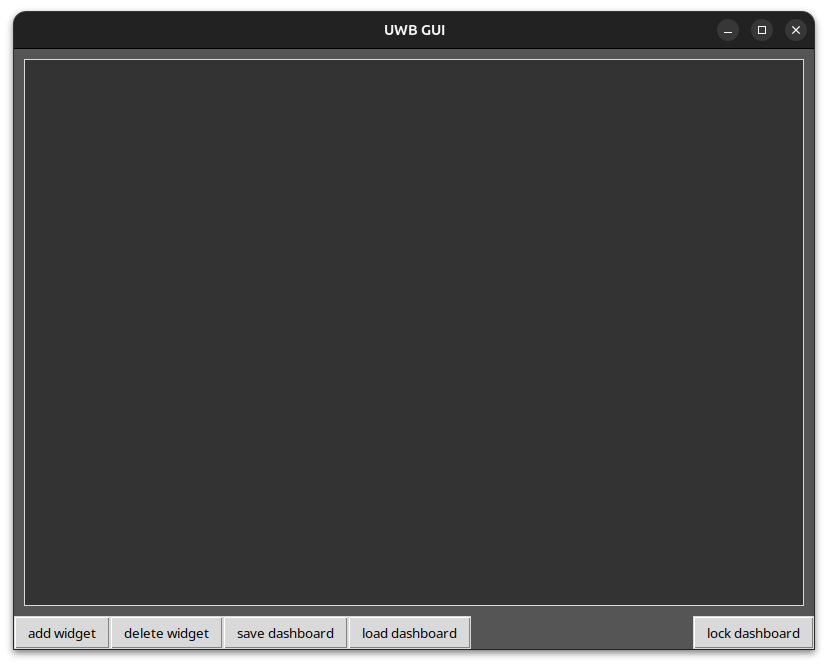
\includegraphics[width=0.65\textwidth]{pictures/gui_idle.png}
	\caption{Empty GUI after startup}
	\label{fig:gui_idle}
\end{figure}



\section{Add a Widget}
Adding a widget is a fundamental action in your dashboard application. Widgets are the building blocks of your dashboard, allowing you to display various types of information and functionality. To add a widget to your dashboard, follow these steps:

Click the "Add Widget" button: Locate and click the "add widget" button on your dashboard's user interface. This action will trigger a dialog or menu to appear like desplayed in Figure \ref{fig:add_widget}.

Select Widget Type: In the dialog or menu, you'll be presented with a list of available widget types. Choose the type of widget you want to add to your dashboard. Your options include "BleServiceWidget", "BleConfigWidget", "SerialWidget" and "BlePlotPositionWidget". 

Confirm and Add: Click the "OK" button to confirm your selection. The selected widget will now be added to your dashboard canvas.

Customize and Position: Once added, you can customize the widget's appearance and content as needed. You can also position it on the canvas by dragging it to your desired location.

Repeat as Needed: You can add multiple widgets to your dashboard following the same process. Each widget can serve a unique purpose and display distinct information.

\begin{figure}[!hbt]
	\centering
	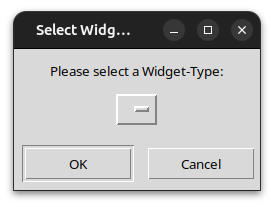
\includegraphics[width=0.35\textwidth]{pictures/add_widget.png}
	\caption{Prompt to add a widget}
	\label{fig:add_widget}
\end{figure}

\section{Remove a Widget}
If you no longer need a widget on your dashboard or wish to rearrange its layout, you can remove it. Here's how to remove a widget from your dashboard:

Click the "Remove Widget" Button: Locate and click the "delete widget" or "remove widget" button on your dashboard's user interface. This action will prompt a dialog or input box.

Specify Widget to Remove: In the dialog, you may need to specify which widget you want to remove. This is typically done by entering the widget's index or selecting it from a list.

Confirm Deletion: Confirm your choice to delete the widget. The selected widget will be removed from your dashboard, and the layout will adjust accordingly.

Optional: You can repeat this process to remove additional widgets as needed.

\begin{figure}[!hbt]
	\centering
	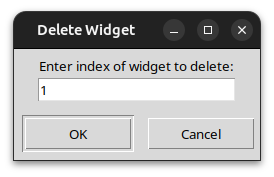
\includegraphics[width=0.35\textwidth]{pictures/delete_widget.png}
	\caption{Prompt to remove a widget}
	\label{fig:delete_widget}
\end{figure}


\section{Save Current Dashboard}
Saving your current dashboard layout and widget configurations allows you to preserve your work for future use. To save your current dashboard, follow these steps:

Click the "Save Dashboard" Button: Locate and click the "save dashboard" button on your dashboard's user interface. This action will initiate the saving process.

\section{Load a Dashboard}
Loading a previously saved dashboard configuration allows you to restore a layout and widget setup. Here's how to load a dashboard:

Click the "Load Dashboard" Button: Locate and click the "load dashboard" button on your dashboard's user interface. This action will load the last saved dashbord onto the user interface.

Continue Editing: You can continue editing and customizing your loaded dashboard as needed.

\section{Lock / Unlock Dashboard}
Locking and unlocking the dashboard is a feature that restricts or enables interaction with the widgets on the canvas. Here's how to lock and unlock your dashboard:

\subsection{Lock Dashboard}
Click the "Lock Dashboard" Button: Locate and click the "lock dashboard" button on your dashboard's user interface. This action will activate the dashboard lock feature.

Widgets Become Static: When the dashboard is locked, all widgets on the canvas become static and unresponsive to user interactions. You cannot move or resize them.

Limited Functionality: Some buttons or features for adding, removing, or configuring widgets may become disabled while the dashboard is locked like the add and remove widget buttons. 

\subsection{Unlock  Dashboard}
Click the "Unlock Dashboard" Button: To regain full interaction with your widgets, click the "unlock dashboard" button on your dashboard's user interface. This action will deactivate the dashboard lock feature.

Widgets Become Interactive: Once the dashboard is unlocked, you can freely move, resize, and interact with the widgets as needed.

Full Functionality Restored: All buttons and features related to widget management become active and usable when the dashboard is unlocked.

Use the lock and unlock feature as needed to control the level of interactivity and customization available for your widgets on the dashboard. This feature can be especially useful when you want to prevent accidental changes to your layout.